\documentclass{beamer}
\usepackage[utf8]{inputenc}
\usepackage[final]{pdfpages}

\usetheme{Goettingen}%Warsaw}
\usecolortheme{lily}
\setbeamertemplate{footline}[page number]
\title[Transactional storage for geo-replicated systems ]{Transactional storage for geo-replicated systems - overview}
\author{Jander Nascimento
\and Liviu Varga}
\institute{Université Joseph Fourier}
\date{\today}
\begin{document}

\begin{frame}
\titlepage
\end{frame}

%\AtBeginSubsection[]
{
  \begin{frame}<beamer>
    \frametitle{Roadmap}
    \tableofcontents%[currentsection,currentsubsection]
  \end{frame}
}

%this is filled up with some sample code (we can remove it anytime)

\section{Introduction}

	\subsection{Overview}
	
		\begin{frame}{Objective}
		
			Build scalable distributed system, improve the availability and reduce response time 
		
	\begin{figure} [H]
		\centering
		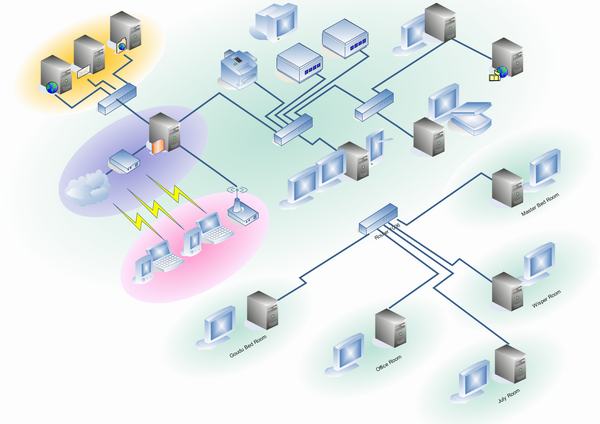
\includegraphics[scale=0.20]{img/fig_network}
	\end{figure}		
		
			How this is achieved?
			\begin{enumerate}
			\item Key-store application
			\item Asynchronous replication
			\end{enumerate}
			
			\begin{block}{Lema}
				Respecting causality order without compromise the throughput
			\end{block}
		
		\end{frame}	
			
		\begin{frame}{Already existing frameworks}
	


		
	
	\begin{columns}
	\begin{column}[1]{5cm}
	
\includegraphics[width=0.5\textwidth]{img/fig_google.png}
	\end{column}
	\begin{column}[1]{5cm}
	
\includegraphics[width=0.5\textwidth]{img/fig_yahoo.png}
	\end{column}
	\end{columns}
		
		
		\begin{figure} [H]
			\centering
			
\includegraphics[scale=0.20]{img/fig_hp}
		\end{figure}				

			Other transaction infrastructure					
		
			\begin{enumerate}
			\item Sinfonia
			\item Percolator
			\end{enumerate}						
					
			Other storage system
			\begin{enumerate}
			\item PNUTS
			\item COPS
			\item Megastore
			\end{enumerate}		

		\end{frame}
	
		\begin{frame}{Dificulties?}
		
		\begin{figure} [H]
			\centering
			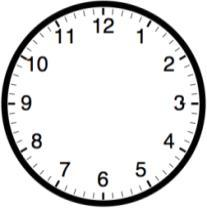
\includegraphics[scale=0.20]{img/fig_clock}
		\end{figure}			
		
		What are the problems faced?		
		
			%talk about sinfonia compare with other the type server that dont use transactions
		\begin{itemize}
		\item Replication between sites
		\item Preserve consistence		
		\item Conflict resolution
		\end{itemize}
		
		\end{frame}		
	
		\begin{frame}{Basis of the solution}

			Delta between Parallel Snapshot Isolation from others?
			\begin{enumerate}
			\item Snapshot Isolation. e.g. percolator
			\item Ignoring primary site constraint. e.g. sinfonia
			\end{enumerate}

			\begin{alertblock}{Nothing as easy as we thought it would be..}
				Snapshot Isolation protocol had to be changed to support multiple site store
			\end{alertblock}
						
		\end{frame}		

\section{Walter framework}

	\subsection{Parallel Snapshot Isolation}
		\begin{frame}{Tools}
		
			%talk about cset and preferered sites
		
			Snapshot Isolation provide the basics for the current PSI protocol
			
			CSet Counts the object operations
			%talk about what is exactly c set
		
		\end{frame}
		
		\begin{frame}{Properties}
		
		The following properties must be maintained:		
		\begin{itemize}
		\item (Site Snapshot Read) All operations read the most recent committed version at the transaction's site as of the time when the transaction began
		\item (No Write-Write Conflicts) The write sets of each pair of committed somewhere-concurrent transactions must be disjoint
		\item (Commit Causality Across Sites) If a transaction $T_{1}$ commits at a site A before a transaction $T_{2}$ starts at site A, then $T_{1}$ cannot commit after $T_{2}$ at any site
		\end{itemize}		
		
		\begin{itemize}
		\item (Site Snapshot Read) All operations read the most recent committed version at the transaction's site as of the time when the transaction began
		\item (No Write-Write Conflicts) The write sets of each pair of committed somewhere-concurrent transactions must be disjoint
		\item (Commit Causality Across Sites) If a transaction $T_{1}$ commits at a site A before a transaction $T_{2}$ starts at site A, then $T_{1}$ cannot commit after $T_{2}$ at any site
		\end{itemize}
		
		\end{frame}	

		\begin{frame}{Anomalies}
		
		Some anomalies that might affect some store systems are:
		\begin{itemize}
		\item Dirty read
		\item Non-repeatable read
		\item Lost update
		\item Short fork
		\item Long fork
		\item Conflict fork
		\end{itemize}		
		
		\end{frame}

		%%%% JANDER SPEACH ENDS HERE
		%%%% LIVIU STARTS HERE

\begin{frame}{Limitations}

			\begin{enumerate}
			\item Short and long fork may happen
			\item Only a single store system per site used for writing
			\end{enumerate}
			
		\end{frame}

		\begin{frame}{PSI and Conflict resolution}
		
		In order to improve conflict resolution, following approaches are used:
		
		\begin{itemize}
		
		\item Preferred sites: Each object is assigned a preferred site where writes to it can be committed without checking other sites for conflicts
		\item Conflict-free counting set objects: csets only allow incrementation or decremental of elements, operation which are commutative  
		
		\end{itemize}
		
		\end{frame}
		
		\begin{frame}{Transaction Durability}
		
		Two kinds of durability can be used:

		\begin{itemize}
		\item Normal
		\item Disaster-safe durability
		\end{itemize}		
		
		\end{frame} 	
		
		\begin{frame}{Site Recovery}
		
		In case of a full site failure, those approaches can be applied:
		\begin{itemize}
		\item Conservative
		\item Agressive
		\end{itemize}		
		
		\end{frame}	 	
			 	
	\subsection{Design}
	 	
 	%talk about 	 	
	 	
		\begin{frame}{Replication}
				
		\begin{itemize}
		
		\item Synchronizing among sites uses vector timestamps
		\item Each site has a local version number indicating the number of transactions in the snapshot
		\item This allows a casual ordering of the events
		
		\end{itemize}
		
		\end{frame}	 	
		

		\begin{frame}{Types of transaction}
		
		\begin{itemize}
		
		\item Fast commit: used for objects which are local to the preferred site, involving two checks (objects are unmodified since the transaction started and unlocked)
		
		\item Slow commit: the preferred site of the object if a non-local one. This involves 2-phases: all the objects are unmodified and unlocked on their site, and after this it goes as a fast commit protocol		
		
		\end{itemize}

		\end{frame}
 	
	 	
\section{Performance}

	\subsection{Results}
	\begin{itemize}
	\item Experimental setup consisting of 4 machines around the world running on Amazon EC2 cloud platform as well as a private cluster
	\item Base performance was evaluated by comparing Walter with a commercial open-source database library, Berkely DB 11gR2 with comparable results
	\item Read throughput is bounded by the RPC performance and scales linearly with the number of sites
	
	\end{itemize}
	
	\subsection{Recap}
	\begin{frame}{Recap...}
	
		\begin{itemize}
		\item \textit{Asynchronous replication across sites.} Replication is done lazily in the background to reduce latency
		\item \textit{Efficient update-anywhere for certain objects.} Counting sets can be updated efficiently anywhere, while other objects can be updated efficiently at their preferred site
		\item \textit{Freedom from conflict-resolution logic}. which is complex to developers
		\item \textit{Strong isolation within each site.} Provided by PSI.
		\end{itemize}
	\end{frame}


\section{Conclusion}

\begin{frame}{Conclusion}

	and our conclusion is...

\end{frame}

\begin{frame}

	\begin{block}{And.. }
	Questions?
	\end{block}

\end{frame}

\end{document}
